%!TEX root = mainfile.tex

\subsection{Full Width at Half Maximum} % (fold)
\label{sub:full_width_at_half_maximum}
	To accurately calculate the FWHM of the galaxies it is essential to model them as extended bodies rather than point sources. To do this the angular size that a galaxy would subtend on the sky is calculated. The first requirement of this is to determine the size of an average galaxy. There have been limited detections of high redshift galaxies and even fewer have had their parameters defined using spectroscopy. Using values based on confirmed galaxies at redshifts of 6 and candidates at higher redshifts %[Ono_FWHM] [Bouwens_FWHM] [Oesc_FWHM] [Jiang_FWHM] the diameter of a galaxy is fixed at 1.5kpc for all redshifts.

	To avoid unnecessarily complex calculations a cosmological calculator\cite{Ned_Calc} is used to calculate the angular scale \si{\kilo\parsec\per ''} at the given redshifts, a plot of these values is shown in Figure~\ref{fig:redshift_vs_angular_size}.
	\begin{figure}[!htbp]
		\centering
			\begingroup\endlinechar=-1
				\resizebox{0.6\textwidth}{!}{%
					% GNUPLOT: LaTeX picture with Postscript
\begingroup
  \makeatletter
  \providecommand\color[2][]{%
    \GenericError{(gnuplot) \space\space\space\@spaces}{%
      Package color not loaded in conjunction with
      terminal option `colourtext'%
    }{See the gnuplot documentation for explanation.%
    }{Either use 'blacktext' in gnuplot or load the package
      color.sty in LaTeX.}%
    \renewcommand\color[2][]{}%
  }%
  \providecommand\includegraphics[2][]{%
    \GenericError{(gnuplot) \space\space\space\@spaces}{%
      Package graphicx or graphics not loaded%
    }{See the gnuplot documentation for explanation.%
    }{The gnuplot epslatex terminal needs graphicx.sty or graphics.sty.}%
    \renewcommand\includegraphics[2][]{}%
  }%
  \providecommand\rotatebox[2]{#2}%
  \@ifundefined{ifGPcolor}{%
    \newif\ifGPcolor
    \GPcolortrue
  }{}%
  \@ifundefined{ifGPblacktext}{%
    \newif\ifGPblacktext
    \GPblacktexttrue
  }{}%
  % define a \g@addto@macro without @ in the name:
  \let\gplgaddtomacro\g@addto@macro
  % define empty templates for all commands taking text:
  \gdef\gplbacktext{}%
  \gdef\gplfronttext{}%
  \makeatother
  \ifGPblacktext
    % no textcolor at all
    \def\colorrgb#1{}%
    \def\colorgray#1{}%
  \else
    % gray or color?
    \ifGPcolor
      \def\colorrgb#1{\color[rgb]{#1}}%
      \def\colorgray#1{\color[gray]{#1}}%
      \expandafter\def\csname LTw\endcsname{\color{white}}%
      \expandafter\def\csname LTb\endcsname{\color{black}}%
      \expandafter\def\csname LTa\endcsname{\color{black}}%
      \expandafter\def\csname LT0\endcsname{\color[rgb]{1,0,0}}%
      \expandafter\def\csname LT1\endcsname{\color[rgb]{0,1,0}}%
      \expandafter\def\csname LT2\endcsname{\color[rgb]{0,0,1}}%
      \expandafter\def\csname LT3\endcsname{\color[rgb]{1,0,1}}%
      \expandafter\def\csname LT4\endcsname{\color[rgb]{0,1,1}}%
      \expandafter\def\csname LT5\endcsname{\color[rgb]{1,1,0}}%
      \expandafter\def\csname LT6\endcsname{\color[rgb]{0,0,0}}%
      \expandafter\def\csname LT7\endcsname{\color[rgb]{1,0.3,0}}%
      \expandafter\def\csname LT8\endcsname{\color[rgb]{0.5,0.5,0.5}}%
    \else
      % gray
      \def\colorrgb#1{\color{black}}%
      \def\colorgray#1{\color[gray]{#1}}%
      \expandafter\def\csname LTw\endcsname{\color{white}}%
      \expandafter\def\csname LTb\endcsname{\color{black}}%
      \expandafter\def\csname LTa\endcsname{\color{black}}%
      \expandafter\def\csname LT0\endcsname{\color{black}}%
      \expandafter\def\csname LT1\endcsname{\color{black}}%
      \expandafter\def\csname LT2\endcsname{\color{black}}%
      \expandafter\def\csname LT3\endcsname{\color{black}}%
      \expandafter\def\csname LT4\endcsname{\color{black}}%
      \expandafter\def\csname LT5\endcsname{\color{black}}%
      \expandafter\def\csname LT6\endcsname{\color{black}}%
      \expandafter\def\csname LT7\endcsname{\color{black}}%
      \expandafter\def\csname LT8\endcsname{\color{black}}%
    \fi
  \fi
  \setlength{\unitlength}{0.0500bp}%
  \begin{picture}(7200.00,4320.00)%
    \gplgaddtomacro\gplbacktext{%
      \put(849,595){\makebox(0,0)[r]{\strut{} 0}}%
      \put(849,947){\makebox(0,0)[r]{\strut{} 0.05}}%
      \put(849,1299){\makebox(0,0)[r]{\strut{} 0.1}}%
      \put(849,1651){\makebox(0,0)[r]{\strut{} 0.15}}%
      \put(849,2003){\makebox(0,0)[r]{\strut{} 0.2}}%
      \put(849,2355){\makebox(0,0)[r]{\strut{} 0.25}}%
      \put(849,2707){\makebox(0,0)[r]{\strut{} 0.3}}%
      \put(849,3059){\makebox(0,0)[r]{\strut{} 0.35}}%
      \put(849,3411){\makebox(0,0)[r]{\strut{} 0.4}}%
      \put(849,3763){\makebox(0,0)[r]{\strut{} 0.45}}%
      \put(849,4115){\makebox(0,0)[r]{\strut{} 0.5}}%
      \put(951,409){\makebox(0,0){\strut{} 0}}%
      \put(2437,409){\makebox(0,0){\strut{} 5}}%
      \put(3922,409){\makebox(0,0){\strut{} 10}}%
      \put(5408,409){\makebox(0,0){\strut{} 15}}%
      \put(6893,409){\makebox(0,0){\strut{} 20}}%
      \csname LTb\endcsname%
      \put(144,2355){\rotatebox{-270}{\makebox(0,0){\strut{}Angular Size}}}%
      \csname LTb\endcsname%
      \put(3922,130){\makebox(0,0){\strut{}Redshift ($z$)}}%
      \put(3922,4022){\makebox(0,0){\strut{}}}%
    }%
    \gplgaddtomacro\gplfronttext{%
      \csname LTb\endcsname%
      \put(3195,3948){\makebox(0,0)[r]{\strut{}$f(x) = 0.024x + 0.113$}}%
    }%
    \gplbacktext
    \put(0,0){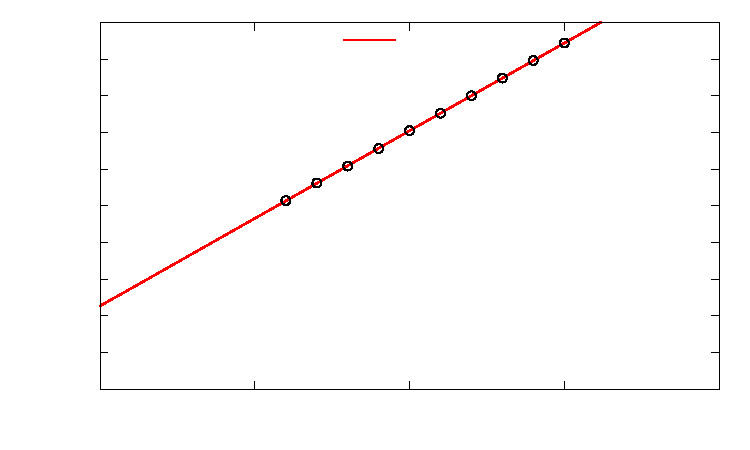
\includegraphics{GRAPH_fwhm_M-ONeill_linear}}%
    \gplfronttext
  \end{picture}%
\endgroup

				}\endgroup
		\caption{A graph showing angular size of target galaxy as a function of redshift.\label{fig:redshift_vs_angular_size}}
	\end{figure}

	This clearly shows a linear trend allowing us to set the FWHM as a simple function of redshift,
	\begin{align}
		\text{FWHM}= 0.0238z + 0.1133
	\end{align}
	this FWHM function then fits into the CCD equation program. This linear trend matches very well with the theory, as is shown in Figure~\ref{fig:angular_size_function_of_redshift}.
	\begin{figure}[!htbp]
		\centering
		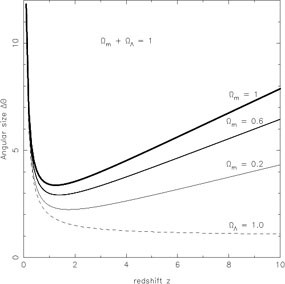
\includegraphics[width=0.5\textwidth]{../Images/angular_size_function_of_redshift.jpeg}
		\caption{A graph showing variation in angular size as a function of redshift\cite{Sahni_FWHM}.\label{fig:angular_size_function_of_redshift}}
	\end{figure}

	Here it can be clearly seen that for the redshifts of interest in this study, between 6--15, the angular size to redshift relation will be in the linear regime. Although this graph does not strictly show $z > 10$, the relation remains linear for a great deal longer and is fully applicable for the majority of the observations proposed in this study.
% subsection full_width_at_half_maximum (end)
